\section{Discussion and Limitations}
\label{sec:discussion}

The quantitative results show a substantial improvement, but understanding the structural limits of CodeGraph is critical for assessing its viability as an agentic retrieval core.

\subsection{Structural Taxonomy of Failures}

An analysis of the 78 zero-recall instances identifies two distinct failure modes that define the boundaries of graph-based retrieval, as illustrated in \Cref{fig:taxonomy}.

\begin{figure}[htbp]
    \centering
    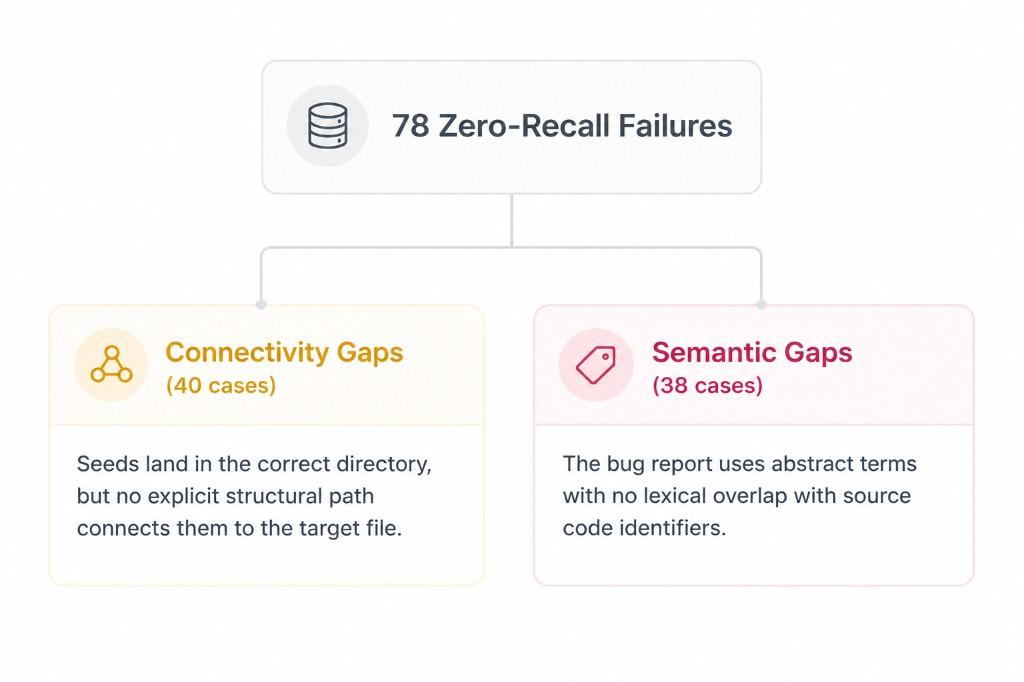
\includegraphics[width=\linewidth]{assets/failure_taxonomy.png}
    \caption{Failure taxonomy of the zero-recall instances. Connectivity Gaps account for 40 cases (missing graph edges). Semantic Gaps account for 38 cases (lexical mismatch).}
    \label{fig:taxonomy}
\end{figure}

\begin{enumerate}
    \item \textbf{Connectivity Gaps (40 instances):} These occur when seeds land in the correct part of the codebase, but no explicit \texttt{CALLS} or \texttt{IMPORTS} edge connects them to the specific target file. Without such a path, Personalized PageRank cannot propagate relevance to the target. This failure mode reflects an inherent limitation of static dependency analysis: files that collaborate through implicit data flows or configuration rather than explicit code imports are invisible to standard structural propagation.
    \item \textbf{Semantic Gaps (38 instances):} These failures arise when the issue description uses abstract natural-language terms with no lexical overlap with any identifier in the source code. For example, a bug described as ``the ORM silently discards null values'' does not contain the code identifier \texttt{\_do\_insert}. Without a lexical match, the system cannot place any seed in the relevant neighborhood, and PPR has no starting point.
\end{enumerate}

\subsection{Ablation: The Cost of Proximity Edges}

To test the limits of the graph schema, we conducted an ablation study where we augmented the graph with \texttt{CO\_LOCATED} edges (connecting all sibling files within the same directory). The intuition was that files in the same directory often collaborate, and such edges might bypass Connectivity Gaps.

However, adding these edges resulted in a regression of 1.0 percentage point. In large, heterogeneous directories, these artificial edges created a dense subgraph connecting unrelated files. Probability mass spread indiscriminately across this subgraph, displacing relevant files from the top ranks. This confirms that CodeGraph's precision derives strictly from high-fidelity dependency-based edges, not from proximity-based heuristics. It is safer to miss an implicit connection than to inject false structural pathways.
